\documentclass[10pt, oneside]{article}   	% use "amsart" instead of "article" for AMSLaTeX format
\usepackage[margin=1in]{geometry}                		% See geometry.pdf to learn the layout options. There are lots.
\geometry{letterpaper}                   		% ... or a4paper or a5paper or ...
%\geometry{landscape}                		% Activate for for rotated page geometry
%\usepackage[parfill]{parskip}    		% Activate to begin paragraphs with an empty line rather than an indent
\usepackage{float}
\usepackage{graphicx}				% Use pdf, png, jpg, or eps§ with pdflatex; use eps in DVI mode
\usepackage{amsmath}
%\usepackage{CJK}	% convert eps --> pdf in pdflatex
\usepackage{achemso}
\usepackage{amssymb}
\usepackage{indentfirst}
\usepackage{url}


\title{Predicting Chemical Properties Using Machine Learning Methods}
\author{Andrew IDs: ccollin1, haichenl, zhonghal}
%\date{}							% Activate to display a given date or no date

\begin{document}
\maketitle

\begin{abstract}

We propose several supervised machine learning based regression models to predict useful properties of chemical compounds, such as molecular orbital energies and band gap. Unlike traditional quantum mechanics based theories which are often computationally infeasible, our machine learning based models take the advantage of chemical similarities between molecules, and have greatly reduced the computational cost by transferring a lot of computational efforts to training stage. To setup our model, we use chemistry knowledge based feature engineering in concert with well-established machine learning regression models such as linear regression, support vector machines, and neural nets. A linear relationship between some of the feature vectors and regression labels can be demonstrated with quantum mechanics perturbation theory. Cross-validated test errors achieved by neural nets model are much lower than some of the state-of-the-art quantum chemistry semi-empirical theories such as INDO, and are even lower than or comparable to the minimum error in experimental measurements, which shows a great potential of practical use in chemistry research.

\end{abstract}



\section{Introduction}
\noindent Quantum mechanics enables us to calculate chemical compounds' properties to a very high accuracy. Unfortunately, such calculations typically involve solving certain nonlinear ill-conditioned partial differential equations, which is extremely time-consuming. For example, to compute the total energy of a given molecule, there are Density Functional Theory (DFT) or \textit{ab initio} theory available for this task; however, they scale $O(n^4)$ to $O(n!)$ asymptotically in CPU time. For a medium-sized molecule that consists of ~100 atoms, one may need tens of hours of CPU time on a modern scientific computing cluster. Often in chemistry research, people deal with chemicals that consist of thousands of atoms (or hundreds of thousands in the case of biochemistry), which requires weeks or months of CPU time. There is thus a need for theories that have better asymptotic scaling rate yet retain an acceptable high level of accuracy. Traditionally, the way to encounter such a dilemma is to introduce approximations in quantum mechanics equations, which leads to Semi-Empirical Quantum Chemistry (SEQC) methods. SEQC methods scale as low as $O(n^2)$, but can only achieve qualitative accuracy. \\

Recent studies show that a variety of machine learning regression models can be employed to predict chemical properties. Instead of solving partial differential equations directly, machine learning models try to predict chemical properties from chemical similarities. From a chemist's point of view, chemicals are made of only a small set of structural building blocks, the properties of which have been thoroughly studied. Molecules consisted of similar building blocks are very likely to share similar chemical properties. Therefore, it is reasonable to train our machine learning models with features come from chemicals made of only a few building blocks, then use these models to predict properties of chemicals that constitute a great number of building blocks. An analogy is to train a spam filter with e-mails that have only a few sentences, and hope that this filter can classify not only short e-mails but also long e-mails that have similar sentences as our training examples do. Unlike quantum mechanical models which are considered ``universal", our models will be, for sure, only applicable to a subset of chemicals, but that is just the inevitable trade-off between accuracy and generality. \\

Philosophically, our feature engineering part is highly related with our chemistry knowledge about our target molecules. It is expected that we are able to extract chemically informative characteristics from every molecule in both training stage and test stage. We have implemented several different ways to transform structural features of all the sample molecules into feature vectors. On the other hand, our training labels are supposed to be generated through DFT calculations. Specifically, we are interested in establishing regression models of the energies of highest occupied molecular orbital (HOMO), lowest unoccupied molecular orbital (LUMO), and band gap. These 3 properties are of great interest in chemistry and physics, both theoretically and experimentally, since they are directly related with molecules' spectroscopic behaviors\cite{hc}. Our goal is to predict these chemical properties with efficient machine learning regression methods, and reduce our error down to ``chemical accuracy", which is numerically equal to 1 kcal/mol or 0.043 eV, and is considered to be the point at which the values calculated are quantitatively significant instead of just qualitatively. Theoretical models that achieve this level of error is typically considered as valid replacements of chemistry experiments that are of great use. \\

In addition, as we mentioned before, in quantum chemistry there exist a lot of SEQC methods that scale significantly better than DFT/\textit{ab initio} but also have systematically larger error rates; yet it is very likely that some machine learning regression models can help us reduce that error if enough training data are given. By employing quantum mechanics perturbation theory, we are able to establish a linear relationship between the properties calculated from SEQC methods and the regression labels calculated from DFT. Detailed discussion about how we utilize SEQC methods in feature engineering can be found later in the feature engineering section. \\

Dataset wise, several types of common polymer chains are constructed as samples; their HOMO, LUMO and band gap (energies) were calculated as labels. We have developed 9 different types of feature vectors to employ supervised machine learning methods, including Linear Regression, Linear Ridge Regression, Support Vector Machines (SVM), K-Nearest Neighbors (k-NN), Decision Tree, Boosting, and Neural Networks. Details on dataset construction, feature engineering, methodology and model developments are demonstrated in the following sections. We present corresponding training/testing errors of combinations of different feature vectors and machine learning models later in the result section. \\




\section{Data and Feature Vectors}

\noindent For this study, 1500 characteristic polymeric systems (chemicals that are built from repeated units, like plastic/rubber/Nylon) were used as training data. These systems are made up from 7 different major building blocks (aryl), (phenyl, furan, vinyl, acetylene, pyrrole, pyridine, and ketone), and 7 minor building blocks, (Hydrogen, methyl, hydroxyl, methoxy, carbenyl, cyano, and amine). All of the polymers used in this study had homogeneous chains of structures to reduce the total size of the dataset. An example polymer structure is shown in Figure ~\ref{furan}. They are divided into one group that consists of Oxygen (O) and another group that consists of Nitrogen (N) for chemical analysis.

Quantum chemistry software package \textit{Gaussian} \cite{gaussian} is applied to compute HOMO, LUMO and band gap at three different DFT levels, namely B3LYP, CAM-B3LYP, and M06HF. These 3 theories have been widely tested in chemical research, and they lead to slightly different numerical results due to how they treat chemical phenomenon differently. In addition to the differing results they yield in these properties, they also produce differing optimized chemical structures (the structures are geometrically optimized to minimize the total amount of chemical strain). From these varied geometries, it is easier to get a more generalized look at how the each of these properties change with slight geometric modifications. This can be seen as analogous to how with image detection researchers will often apply warping filters to their images to populate their dataset with more unique samples. Along with the initial non-optimized geometrical structure, we have 4 types of structures; combining with the aforementioned 3 DFT theories, we have essentially obtained 12 data sets that contain slightly different information, yielding $\sim12000$ unique data points (with more structures still being calculated with DFT).


\begin{figure}[H]
\begin{center}
\includegraphics [width=.3\textwidth]{furan.png}
\caption{An example polymer structure of consisting of 4 furan backbone sections with hydroxyl and methoxy for the R groups.}\label{furan}
\end{center}
\end{figure}

% \begin{figure}[hb]
% \begin{center}
% \includegraphics [width=1\textwidth]{orbital.png}
% \caption{Example HOMO (left) and LUMO (right) orbitals}\label{orbital}
% \end{center}
% \end{figure}

The following part shows how we extract 11 types of feature vectors from each structure based on chemical intuition:

\begin{enumerate}
\item \textbf{Null}: An empty list that serves as the worst result to compare against. This feature vector also is used to compare the amount of error that is contained implicitly in each of the different datasets between all of the DFT methods. Effectively, this feature vector is just the metadata about the datasets which will be mentioned later.

\item \textbf{Binary}: It creates a simple boolean feature vector based on whether or not a building block exists in the structure. Mostly speaking, we only consider the existence of aryl-group and r-group. For example, it turns each building block into 1 or 0 in. This works similar to the binarization of a corpus of words as seen often with text based machine learning.

\item \textbf{Flip Binary}: This is similar to the binary feature vector, except that for each aryl group that appears in the structure, it takes into account whether or not the ring was rotated 180 around the connecting bond between the two units. When dealing with conjugated systems, like we have, the rotations can have a significant effect. This vector takes that into account by adding an extra binary feature for each link in the chain.

\item \textbf{Decay}: This feature vector makes the approximation that the relation between all of the atoms/structures within the molecule have some sort of a intrinsic decay, (atoms infinitely far apart should not influence each other). For this, the first aryl group in the chain is considered the zero point (influence of 1), and all the subsequent aryl groups influences are defined by a decay function $ W = \sum_{i} (Ad_{i}^{-H})^{p}$, where $A$, $H$, $p$ are constant factors to determine rate of decay, $d_{i}$ is the distance from the $i$th group. This feature also has the added benefit that it has $O(1)$ space requirements compared to the normal binary feature vector which is $O(N)$ where $N$ is the number of aryl groups.

\item \textbf{Gaussian Decay}: This feature vector came about after examining the PCA results of the weights of a linear regression. After looking at the relative influence of each of the polymer features in the binary vector, it was found that the decay as the length of the chain got longer was closer to a Gaussian decay that just a power decay. This feature was used as an attempt to match that new data. $W = \sum_{i} e^{-\left(\frac{x}{\sigma}\right)^2} $. Where $\sigma$ is just another parameter to tune to match the decay.

\item \textbf{Centered Decay}: This feature vector takes the same approach as the decay feature vector with the addition that it does the decay from the center of the structure using a radial distance rather than just starting from one end.

\item \textbf{Signed Centered Decay}: This works similar to the centered decay feature vector with the addition that it takes into account the side of the center that the rings are on instead of just looking at the magnitude of the distance.

\item \textbf{Coulomb}: This feature vector is based on the work in Hansen et. al \cite{Hansen}. It consists of a distance matrix between all of the atoms in the structure with each element multiplied by the number of protons in each of atom in the pair. The diagonal elements based on a fit that that Hansen et. al did to match atoms to different properties. While this feature vector generalizes well, it scales $O(N^2)$ with respect to the number of atoms in the structure.

$$
 C_{ij} =
  \begin{cases}
       0.5 Z_i^{2.4} & : i = j \\
    \frac{Z_i Z_j}{| r_i - r_j |} & : i \neq j \\
  \end{cases}
$$

\item \textbf{PCA Coulomb}: This feature vector takes the feature matrix from coulomb feature and does Principal Component Analysis on it to extract the N most influential dimensions. The goal of this is to reduce the size of the feature vector which can reduce overfitting, and most importantly dramatically reduce running time. This is specifically applied to the coulomb feature vector because of its poor scaling as the polymers get larger. For this study we looked at just the 100 most influential layers.

\item \textbf{Fingerprint}: This feature vector takes looks at all the functional groups in a structure and generates a semi unique ``fingerprint". In theory, this feature vector should work for any structure, not just polymers and it does not have the same sort of scaling issues as the coulomb matrix.


\item \textbf{SEQC Feature Engineering}:
Eventually (and formally), for HOMO and LUMO energies, we want to solve the quantum mechanics 1-electron Sch\"{o}dinger equation. If there are $m$ electrons in the system, the equation for the $i$th electron is:
\begin{flalign*}
H^{DFT}(\psi_1,\cdots,\psi_m)\psi_i &= \epsilon_i \psi_i
\end{flalign*}
Where $H^{DFT}(\psi_1,\cdots,\psi_m)$ is the 1-electron DFT Hamiltonian operator that characterizes a single electron's total energy; notice that this operator depends on $\psi_1,\cdots,\psi_m$, i.e. its solutions. $\psi_i$ is the wavefunction (orbital) of the $i$th electron, and $\epsilon_i$ is the energy of the $i$th electron. Accordingly, there are in total $m$ equations, one for each electron. Our regression labels $E_{HOMO}$ and $E_{LUMO}$ are defined as:
\begin{flalign*}
E_{HOMO} &= \epsilon_m \\
E_{LUMO} &= \epsilon_{m+1}
\end{flalign*}

In plain English, $E_{HOMO}$ is the energy of the electron which has the highest energy in the molecule, and $E_{LUMO}$ is the lowest ``virtual" energy of the unoccupied electron orbitals. The regression label $E_{\text{Band Gap}}$ involves many-electron Sch\"{o}dinger equation and is therefore not suitable to be described here, but a clue is that $E_{\text{Band Gap}}$ depends on all $\psi_i$'s and $\epsilon_i$'s. \\

If we expand $H^{DFT}(\psi_1,\cdots,\psi_m)$ and $\psi_1,\cdots,\psi_m$ in $n$ basis functions, the problem is turned into solving a non-linear algebraic equation system, and we can write the $m$ equations compactly in matrix form as:

\begin{flalign*}
\bold{H^{DFT}(C)C} &= \boldsymbol{\epsilon}\bold{C}
\end{flalign*}

$\bold{C}$ is a unitary matrix where each column is an eigenvector of $\bold{H^{DFT}(C)}$, and $\boldsymbol{\epsilon}$ is a diagonal matrix consisting of all the eigenvalues (energies) $\epsilon_i$'s. \\

The Hamiltonian operators of SEQC methods possess similar forms as DFT Hamiltonians do. The corresponding matrix equation can be written as:

\begin{flalign*}
\bold{H^{SEQC}(C')C'} &= \bold{E}\bold{C'}
\end{flalign*}

Where $\bold{C'}$ consists of SEQC eigenvectors, and diagonal matrix $\bold{E}$ consists of SEQC electron orbital energies $E_i$'s. \\

Suppose we have solved an SEQC matrix equation; now we have known all the $E_i$ values, and we essentially have obtained a linear transform from the original Hilbert space spanned by the $n$ basis functions to the solution space spanned by linear combinations of the $n$ basis functions, the combination coefficients being elements of $\bold{C'}$; denote these new basis functions as $\Phi_i$'s. We then try to solve DFT equations in the new Hilbert space. According to quantum mechanics perturbation theory, such a solution can be expanded by a Taylor series (if we ignore terms with order higher than 2):

\begin{flalign*}
\epsilon_i &= \epsilon_i^{(0)} + \epsilon_i^{(1)} + \epsilon_i^{(2)} + \cdots \\
\end{flalign*}

Where:
\begin{flalign*}
\epsilon_i^{(0)} &= E_i \\
\epsilon_i^{(1)} &= <\Phi_i|H^{DFT} - H^{SEQC}|\Phi_i> \\
\epsilon_i^{(2)} &= \sum_{j\ne i}{\frac{|<\Phi_i|H^{DFT} - H^{SEQC}|\Phi_j>|^2}{E_i - E_j}} \\
\end{flalign*}

The 0th order term tells us that $E_i$ gives us a qualitative estimation of $\epsilon_i$, so that we can directly use $E_i$'s that come from different SEQC methods as part of our feature vector. Further, since the molecules we are using are chemically similar to each other, there is a reason to think that $\Phi_i$'s on different molecules are similar to each other as well. We therefore assume that $|<\Phi_i|H^{DFT} - H^{SEQC}|\Phi_j>|^2$ values on different molecules are close enough to each other as well. In such a sense, the 2nd order term can be viewed as a linear combination of $\frac{1}{E_i - E_j}$ values. Since these values asymptotically go to 0 when $E_i - E_j$ becomes large, we pick up an orbital cutoff as well. Specifically, we select $E_{m-4} \sim E_{m+4}$ orbital energies calculated with different SEQC methods, and take the 2nd term $\frac{1}{E_i - E_j}$ values as part of our feature vector. \\

\end{enumerate}

To take into account the different datasets, an extra bit of meta data is attached to the end of each of the feature vectors. The first part is a four component boolean vector that indicates which method was used to optimize the structure (either ``non-optimized", ``B3LYP", ``CAM-B3LYP", or ``M06HF"). The second part consists of three boolean values that indicate the final DFT method that was used to calculate the molecular properties (``B3LYP", ``CAM-B3LYP", or ``M06HF"). Finally, all of the feature vectors then have an extra bias term added to the end. In the case of the null feature vector this is the entirety of the data that is contained.





\section{Machine Learning Algorithms and Methodology}

\noindent For the implementations of the various machine learning algorithms, we choose to use the Python package SciKit-Learn \cite{scikit-learn}. Specifically we applied Linear Regression, Linear Ridge Regression, Support Vector Machines (SVM), K-Nearest Neighbors (k-NN), Decision Tree, Boosting. We have implemented our own interface routines in order to fulfill our needs and to communicate with \textit{Gaussian} quantum chemistry package.

To pick the best hyperparameters for each of the models, they all underwent two layers of k-folds cross validation (5 folds for outer layer and 2 folds for inner layer). The outer layer was used to set aside the test set, and the inner was used to cross validate for all of the hyperparameters in the models, as shown in Figure ~\ref{crossvalidation}. To minimize the time spent cross validating and maximize the range of values tested, the hyperparameters were scanned on a log scale (with the exception of k-nearest neighbors and tree regression which used Fibonacci spacing). The hyperparameters that produced the lowest errors in cross validation were then used on the test set to get the final results.

\begin{figure}[H]
\begin{center}
\includegraphics [width=0.4\textwidth]{crossvalidation.png}
\caption{A simple diagram of the overall cross validation/testing process.}\label{crossvalidation}
\end{center}
\end{figure}

Along with the more straightforward methods, neural networks were utilized to try to predict the molecular properties. For the neural networks, we utilized the Python library PyBrain\cite{pybrain}. Because neural nets allow parallel outputs, the neural nets were all trained using all three properties at the same time to produce a single model. This directly contrasts with the other methods which required a model for each property. More on the significance of this will be discussed in the conclusion. In the interest of time, only the flip binary feature vector was used when training the neural nets. This feature vector was picked due to its strong performance with all of the other machine learning methods.

Specifically, for the neural nets, selecting the correct architecture is a big concern. For this task, a similar method of cross validation was done with 80/20 splits for training/testing. A brute force search was done for the best performing architecture using layers of 10, 20, 40, 80, and 160 nodes per hidden layer. This was carried out for the first two layers. For the third layer, only the best performing first two layers were considered. As an overall trend increasing the size of each layer improved the total error log linearly, but greatly increased the total amount of time required to train the neural net. When trying to decide on the best architecture, all of the neural nets were compared based on their testing error after 1000 generations. This was done to not give an advantage to smaller networks that could otherwise train for longer because of their reduced computational cost. Also, by this point, the neural nets had settled into their standard $err = a t^{-b} $ rate of decay.



\section{Results and Interpretation}

\noindent We have plotted the test results versus different machine learning methods for various features in Figure ~\ref{homo}, Figure ~\ref{lumo} and Figure ~\ref{gap}. These results show that all the machine learning algorithms run well on our feature vectors and predict reasonable values for HOMO, LUMO, and band gap. In all figures, the prediction errors from other machine learning algorithms are well below the ``mean" method, indicating that these methods work better than random guess. For a certain algorithm, prediction errors from all features that we have developed are all significantly lower than null feature, which shows that our feature extraction also works better than just making predictions based on which dataset the structure came from. SVM and Decision Tree methods already show particularly low test errors and can be utilized for chemical calculation to some extent.


\begin{figure}[H]
\begin{center}
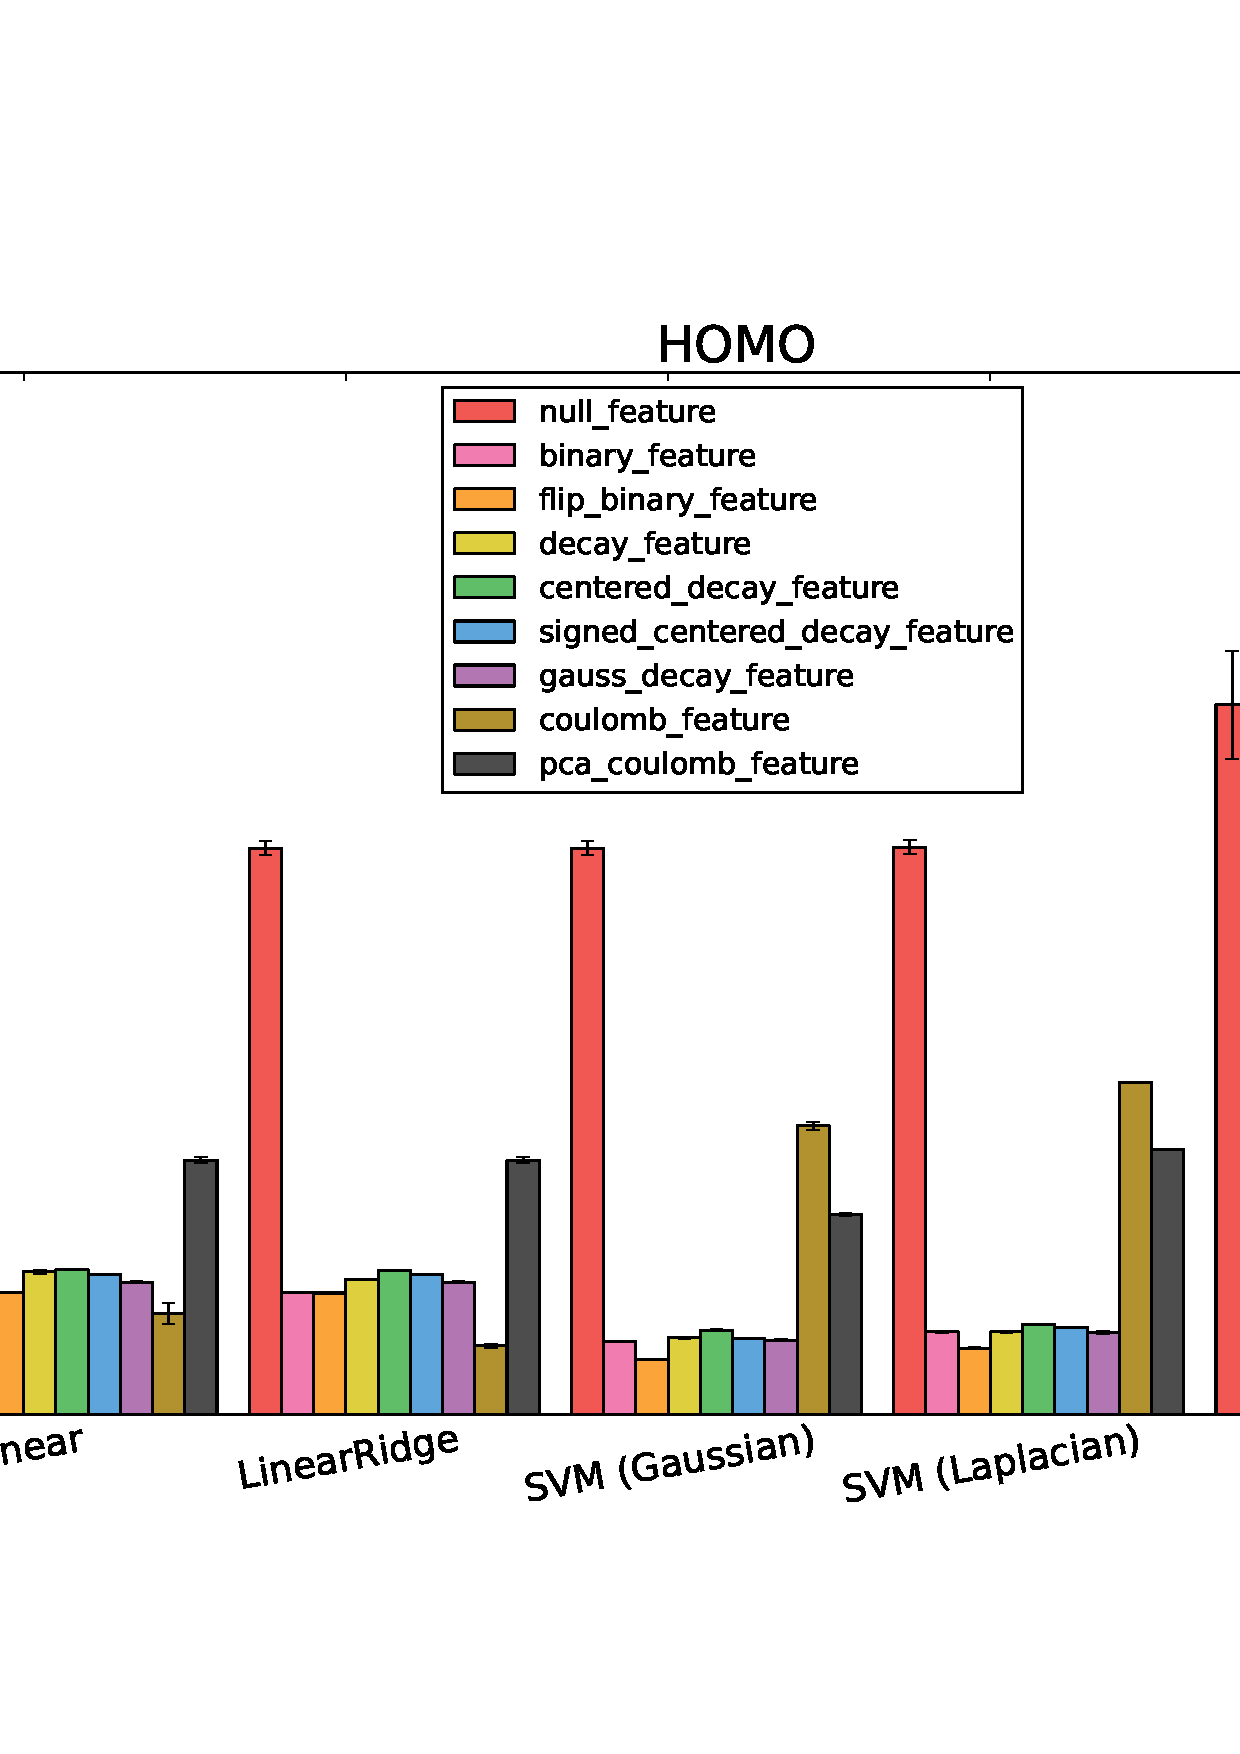
\includegraphics [width=.8\textwidth]{homo_results.png}
\caption{The HOMO test errors for each of the different methods/vectors.}\label{homo}
\end{center}
\end{figure}

The lowest errors can be seen with the SVM with Gaussian kernels. Most of the feature vectors perform similarly with each machine learning algorithm implying that, as a whole, the algorithm is more influential than the data representation which correlates with the results seen by Hansen et. al. Between the properties, the LUMOs had the lowest errors with the HOMOs being slightly higher. The highest of all the errors were seen with the band gaps. These can all be explained chemically in the fact that the HOMO and LUMO are more directly related to the structure of the molecule, whereas the band gap is a combination of many secondary effects as well as the structure.

\begin{figure}[H]
\begin{center}
\includegraphics [width=.8\textwidth]{lumo_results.png}
\caption{The LUMO test errors for each of the different methods/vectors.}\label{lumo}
\end{center}
\end{figure}

Unfortunately, the results for the fingerprint feature vector could not be included due to a bug in the chemical fingerprint library which caused some of the the structures with Nitrogen to not work. Because of this they were excluded because they can not be directly compared against. The general trend seen with just the Carbon, Hydrogen, and Oxygen dataset was that the fingerprint feature vector outperformed the flip binary feature slightly.

\begin{figure}[H]
\begin{center}
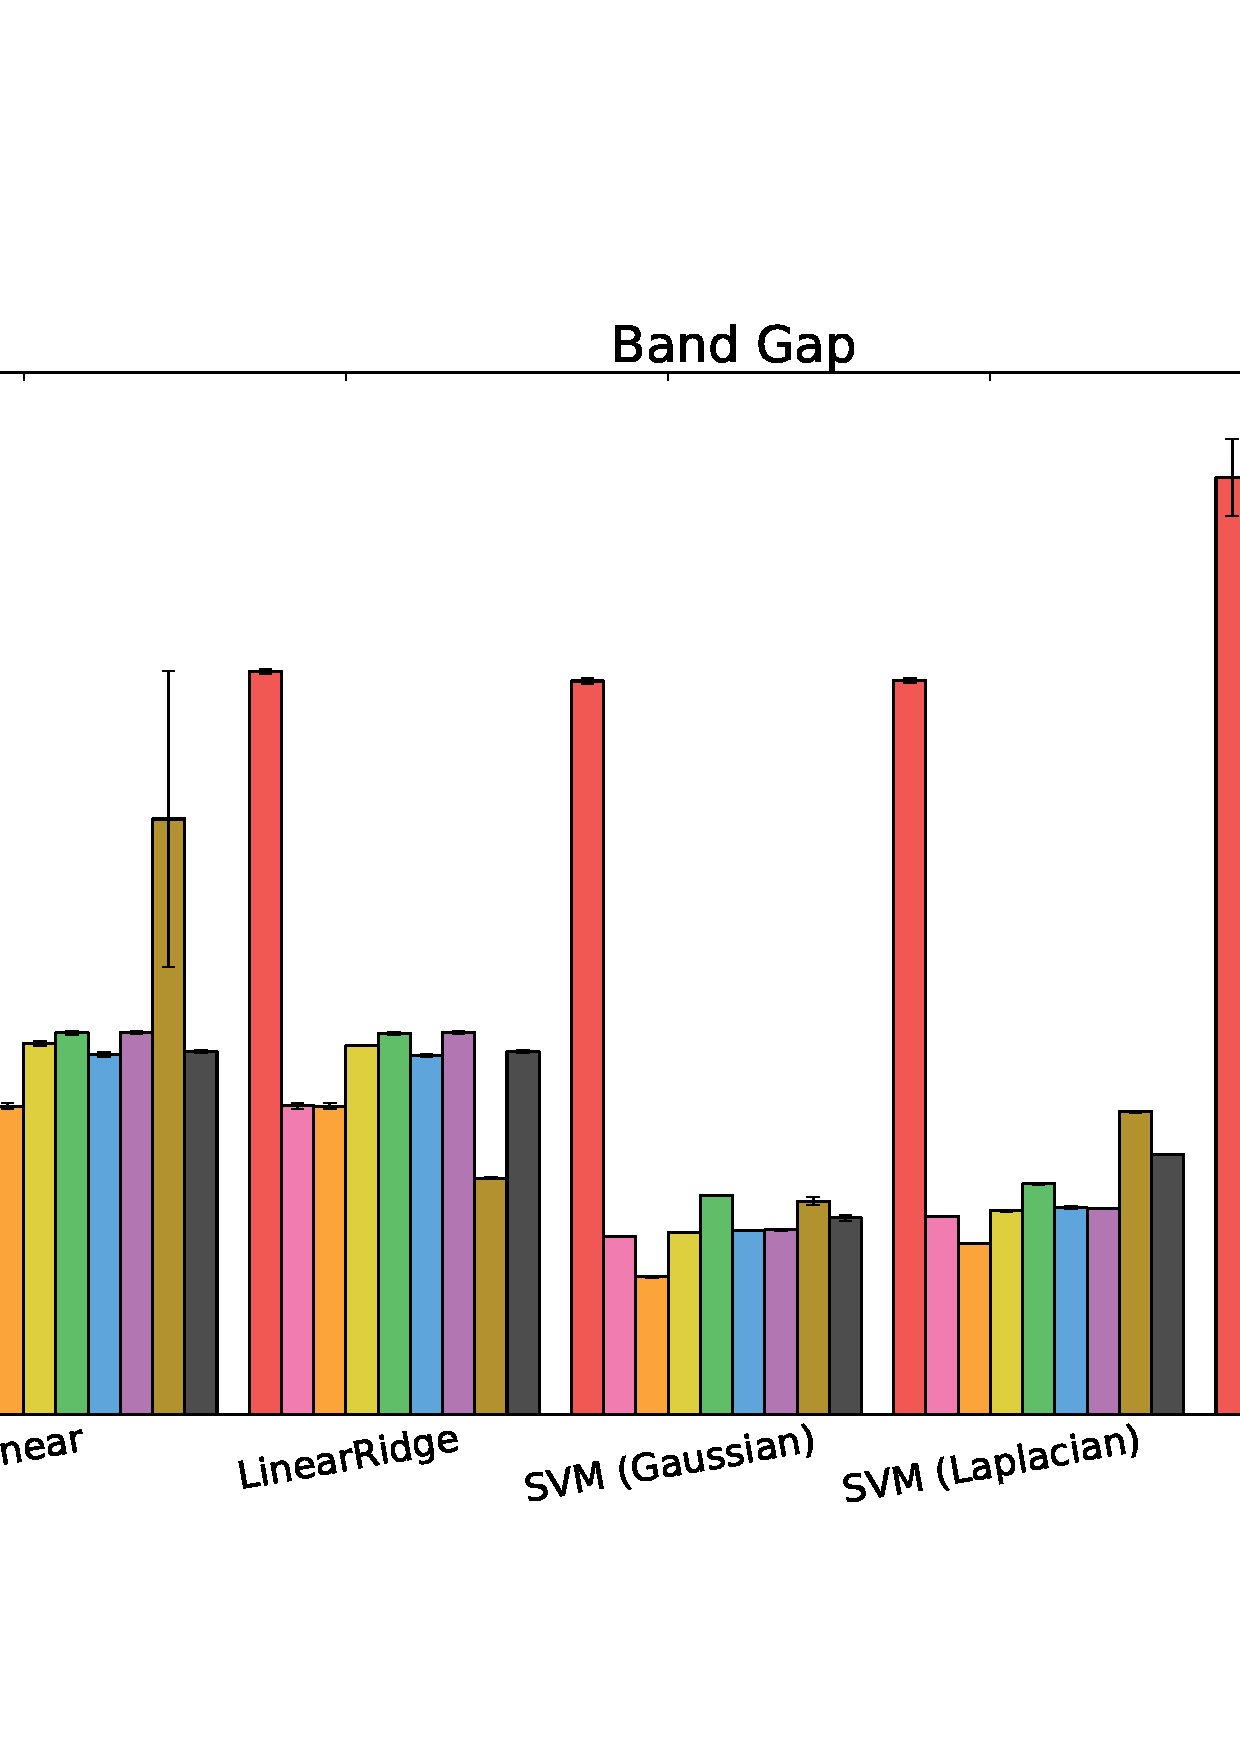
\includegraphics [width=.8\textwidth]{gap_results.png}
\caption{The band gap test errors for each of the different methods/vectors.}\label{gap}
\end{center}
\end{figure}

The flip binary feature vector has the best performance of all the feature vectors. This can be attributed to two factors, 1) it contains more relevant information than the binary feature, so it will quite readily out perform it. 2) This implies that the decay function used in the decay feature vectors is not a good representation of the physical relation between the structures. It may also be possible that this discrepancy stems from the fact that the polymer chains that were used for this study were all fairly short. Further work will have to be done with longer polymers to confirm this.

Unexpectedly, the Coulomb feature vector did not perform better with the Gaussian kernel than with the Laplacian kernel as expected from the work by Hansen et. al\cite{Hansen}. And more than that, as a whole the Gaussian kernel outperformed the Laplacian kernel. The only intuition in to why this might be the case is that the structures used are all highly conjugated, which means that electrons are allowed to flow more freely than in less conjugated systems like what Hansen et. al tested on.

Overall, the neural nets were able to produce the lowest errors for all three properties. This is due in part to two main factors. The first of which being that they are a very general method. The second main factor is that they are able to exploit the inter relation between all three of the properties in this study. Roughly speaking, the band gap can be predicted from the HOMO and the LUMO. With this relation, the neural net is able to produce much better results than the other methods. A similar improvement can be seen with the inclusion of the other properties in the feature vector as seen with the SEQC Feature Engineering in Figure ~\ref{seqc}. From this plot it is readily apparent that the inclusion of the properties as predicted by semi empirical methods can reduce the error 20-30\%. This amount of a difference could be used to explain at least part of why the neural nets performed better.

\begin{figure}[H]
\begin{center}
\includegraphics [width=.7\textwidth]{seqc_fig.png}
\caption{The band gap test errors for each of the different methods/vectors.}\label{seqc}
\end{center}
\end{figure}

What is even more interesting is that the best performing neural net in this study, the 105x80x40x20x3 sigmoid, performs quite a bit better than an equivalent semi empirical method, INDO. These results can be seen in Figure ~\ref{NN-indo}. Along with just the numerical results of the errors, we also looked at the evolution of the property gradient as each of the data points progressed through the neural net as can be seen in Figure ~\ref{nnpca}. As can be seen in the figure, the total gradient of the image becomes smoother and clearer.

\begin{figure}[H]
\begin{center}
\includegraphics [width=.8\textwidth]{neural-default-indo.png}
\caption{Neural Networks compared to INDO. The top row of plots show how well the neural nets and INDO results match to DFT (along the diagonal means perfect correlation). The bottom row of plots show the distribution of errors. The banding that can be seen in the INDO results is due to the differences in the results of the DFT methods. The neural net does not have this same kind of banding because this metadata is included in the feature vector.}\label{NN-indo}
\end{center}
\end{figure}

\begin{figure}[H]
\begin{center}
\includegraphics [width=.9\textwidth]{nnpca.png}
\caption{PCA each of the layers of a 105x80x40x20x3 Neural Network from the input on the left to the output on the right. The plots in the box correspond to the hidden layers (The upper being the first linear transformation, and the plot directly below after the application of the sigmoid function). The color corresponds to the HOMO value. Red signifies higher values and blue corresponds to lower values. The nice gradient on the right indicates that the the overall fit worked.}\label{nnpca}
\end{center}
\end{figure}

Neural Networks produce 0.027, 0.026, and 0.036 eV errors for HOMO, LUMO, and Band Gap respectively, which are much lower than the chemical accuracy 1 kcal/mol (0.043 eV). These errors together with the speed at which these predictions can be made make neural networks by far the best method. A few other kinds of neural nets were tried (such as tanh layers and recurrent networks), but they did not have the same level of performance as the simple forward feed network with sigmoid layers.


\section{Conclusion and Future Directions}

Overall, all of the machine learning methods and all of the feature vectors performed fairly well. This implies that perhaps many of the problems seen in computational chemistry today can be solved with the proper application of machine learning. Of all feature vectors, the flip binary feature vector worked the best for all of the algorithms. For the methods themselves, the neural nets performed the best by quite a large margin (0.027, 0.026, and 0.036 eV for HOMO, LUMO, and Band Gap respectively).

What is especially nice about neural nets is that they are able to generalize well to many kinds of datasets and they are very simple in both implementation and parallelization. Because of these factors they are significantly faster than the more complex semi semi empirical methods (about 20,000 times faster than INDO). The neural net predictions take on the order of seconds for all 12,000 structures, whereas the INDO calculations take on the order of tens of hours. Both of these, however, are dwarfed by the total amount of time that has been required to generate the DFT data. Which is on the order of a quarter of a million CPU hours. When compared to DFT, the neural nets are a massive time saver by being about 350,000,000 times faster.

In the future, more work needs to be done on the neural nets, both in scale, technique, and in what kinds of neural networks. It is reasonable to assume to assume that larger layers will produce lower error rates due to the trend found when exploring different architectures. It is suspected that an architecture similar to a convolution network might work really well for this kind of data due to the locality of the chemical structures (and the similarity of how the functional groups act in a structure).

For more of a traditional machine learning approach, more work can be done to incorporate multi output methods to take advantage of the inter relation between the different properties. Also,more work can be done with the standard methods by doing more work with the SEQC feature vector to attempt to make up for the lack of cross information between the properties when training separately.

Another direction that could be explored is the inclusion of other molecular properties such as total energy, dipole, quadrapole, and etc. As with any project, more data can always be added, but in this case the increase in data should correspond to the inclusion of other kinds of atoms (S, F, P, and etc). Unfortunately, the chemical fingerprinting did not work for the nitrogens due to a technical issue with the conversion of atomic coordinates and bond information. More work will need to be done to track down what caused the issue. Lastly, and maybe the most important would be to generalize these methods such that they could be used with nonpolymeric systems. This problem could be solved with the usage of (working) chemical fingerprints.


\nocite{gaussian}
\nocite{hc}
\nocite{scikit-learn}
\nocite{Hansen}
\nocite{scipy}
\nocite{rdkit}
\nocite{matplotlib}
\nocite{numpy}
\bibliography{final}
\end{document}
